\documentclass[10pt]{report}
\usepackage{epsf}
\usepackage{amsmath}
\usepackage{amssymb}
\usepackage{float}
\usepackage{palatino}
\usepackage[pdftex]{graphics}
\usepackage{fancyhdr}
\usepackage[pdftex]{graphicx}
\usepackage{hyperref}
\parindent 0in
\parskip 1ex
\oddsidemargin  0in
\evensidemargin 0in
\textheight 8.5in
\textwidth 6.5in
\topmargin -0.25in

\pagestyle{fancy}
\fancyhf{}
\fancyhead[L]{\bf BME354L - Palmeri - Spring 2013}
\fancyhead[R]{{\bf Arduino Project}}
%\fancyfoot[L]{LICENSE: CC BC-NC-SA 3.0 ({\tt http://creativecommons.org/licenses/by-nc-sa/3.0/})}
\fancyfoot[C]{\thepage}

\title{Designing Control Systems?}
\author{Will Scheideler}
\begin{document}

\section*{Designing Control Systems}

\par  By now, you have encountered several control systems in BME354 lab such as the baby incubator. The baby incubator is an excellent example because it demonstrates all the key features of a simple control system: an output (controlling the heater), an input (the temperature reading), and some sort of feedback algorithm to relate output to input.

\par The baby monitor is a simple feedback-based control system in that the feedback is based only on the binary state of the output (above or below the set temperature), producing an output which oscillates about the set point. Control systems are present in many devices that you use daily, some of which are much more complex. Air conditioner systems use control systems to set the correct temperature of a room. An elevator uses a control system to smoothly bring the cabin to level with the destination floor. Quadrocopters use advanced control systems to stabilize properly and perform aerial maneuvers and are also used in research applications to test novel control algorithms. In the future, control systems will be used in applications like driverless cars. These are only a few examples-there are even more nuanced applications of control system you probably wouldn't think of, but they are everywhere.

\subsection*{How does a control system work? }

\par Control theory is a vast and deep subject which you could take many courses in, so here we will briefly cover how a control system works. There are many implementations of control systems-the one you implemented in the baby monitor lab is a primitive example. One of the standard mechanisms used is called \textbf{Proportional-Integral-Derivative}, or PID control. PID control, illustrated in the control diagram shown below, is an extremely popular class of control systems. In fact, PID is the most common controller used by industry.

\begin{figure}[H]
\centering
   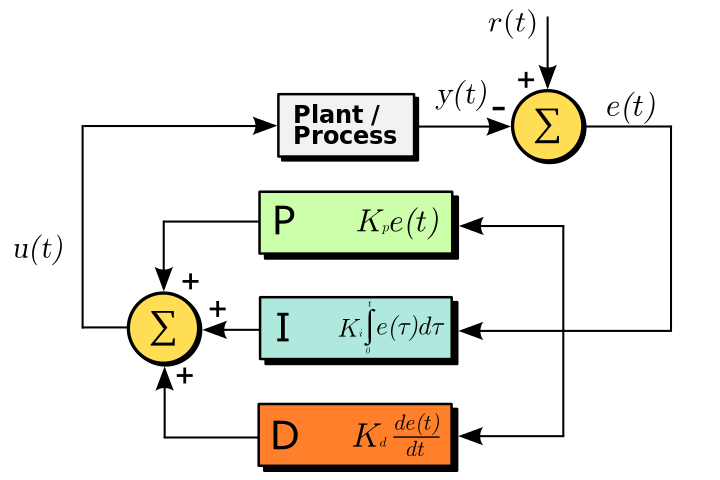
\includegraphics[width=0.7\textwidth]{PID.png}
    \caption{PID Control Diagram}
\end{figure}

\par Your feedback loop is based on three terms: the error between the desired value and the current actual value (proportional control), the total amount of error that has occurred up until now (integral control), and the rate of change of the error (derivative control). Each has a weighting scalar that you can change to control how much each of them affects the output of the system. Using these parameters, you can control how quickly the system will adapt to reach the desired set point, how much the system overshoots, and whether the system oscillates. There is a lot of math that goes on behind the scenes that you will learn if you take a control systems course, but won't be covered here.

\subsection*{How to design a controller for a reflow oven?}

\par In this project, aside from user interface, the primary task will be to design the control system. Although Arduino has made this process a lot easier for you through built-in libraries, there are still some design decisions you will have to make.	

\begin{itemize}
\item What are the relevant temperature resolutions? How accurately can your system measure temperature? Is the resolution closer to $1 ^{\circ}{\rm C}$ or $0.1 ^{\circ}{\rm C}$? How does this affect your control system? Is it even necessary for our application to get $ 0.1 ^{\circ}{\rm C}$ resolution?

\item 
What are the relevant time scales? How quickly do you need your input and output to change? How fast do you need to sample the temperature? This part of the design process is akin to deciding how fast you need to sample a biosignal. Just like a biosignal (which you have seen is not very well band-limited), the time scales / relevant frequencies in this system may not be clear cut. 
	\begin{itemize}
		\item 
		What phenomena would affect this time scale? This is a good time to note that diffusive heat transport has ${t}_D \sim L^2$. If you have taken / are 			taking BME 307 then you recognize this as a time scale for chemical diffusion. 
		\item
		What would convective transport (i.e. using a fan in the reflow oven) do to the time scales that you have to worry about?
		\item
		For the scale of the reflow oven, this means that temperature still fluctuates on a relatively slow time scale (s to 10’s of seconds).
	\end{itemize}

\item 	Is a constant sampling rate the best way to handle your measurements? Could you use a higher precision technique during periods of change? Think about how oversampling / averaging could help improve accuracy.

\end{itemize}

\subsection*{Arduino PID Tutorials}

\par Luckily, there are built-in libraries for Arduino that you can use. Watch the following videos to get started using them.
\begin{itemize}
\item PID Controller Intro: 
\url {http://www.youtube.com/watch?v=UR0hOmjaHp0}
\item PID Control Examples:
\url{http://www.youtube.com/watch?v=XfAt6hNV8XM}
\end{itemize}

\end{document}